% !TEX root =./main.tex

\section{Signal $x_3$}

Signal $x_3$ contains data from an electrocardiogram (ECG) that was contaminated with an artifact from a power line.  Important to note, though, is that the ECG was recorded in Europe, and that European power lines oscillate at $50 \unit{Hz}$, rather than the American $60 \unit{Hz}$.  The contaminated data can be seen in Figure \ref{fig:x3}.

\begin{figure}[H]
    \centering
    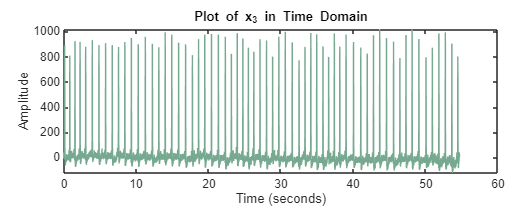
\includegraphics[width=0.5\linewidth]{figures/x3.png}
    \caption{Signal $x_3$ over Time}
    \label{fig:x3}
\end{figure}

Focusing in on the first 15 seconds, as is done in Figure \ref{fig:x3_zoom}, yields a clearer picture of the contamination.
\begin{figure}[H]
    \centering
    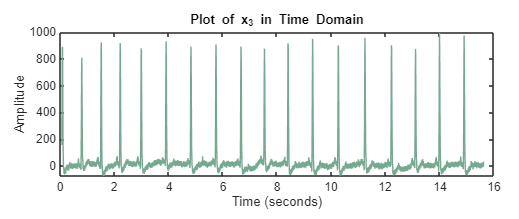
\includegraphics[width=0.5\linewidth]{figures/x3_prefilter.png}
    \caption{Signal $x_3$ over the First 15 Seconds}
    \label{fig:x3_zoom}
\end{figure}

Additionally, looking at the signal's frequency spectrum in Figure \ref{fig:X3} reveals the large magnitude spike around $50 \unit{Hz}$.  This is the contamination that must be removed.
\begin{figure}[H]
    \centering
    \includegraphics[width=0.5\linewidth]{figures/X3_prefilter.png}
    \caption{Frequency Spectrum of Signal $x_3$}
    \label{fig:X3}
\end{figure}


Before designing a filter to remove the contamination, it will be helpful make some measurements.  As can be seen in the markings in Figure \ref{fig:X3_marked}, we see that the peak of the interference is at $-10 \unit{dB}$, while the average if the data is around $-55 \unit{db}$ near $50 \unit{Hz}$.  This requires a filter to decrease the spike's magnitude by about $-45 \unit{dB}$.  Additionally, we can note that the peak is at around $49.8 \unit{Hz}$, and impacts the range of about $48.6 \unit{Hz}$ to $51 \unit{Hz}$.

\begin{figure}[H]
    \centering
    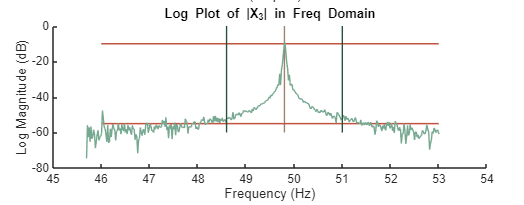
\includegraphics[width=0.5\linewidth]{figures/X3_prefilter_zoom.png}
    \caption{Frequency Spectrum of Signal $x_3$ focused on Interference}
    \label{fig:X3_marked}
\end{figure}

In this signal, preserving linear phase is important to not disrupt important information.  This requires the use of an FIR filter.  Additionally, we will be using a bandstop filter to reduce the magnitude of the interference. Iterating from the starting point given by the measurements conducted earlier, Filter 1 was developed.  The frequency response of Filter 1 can be seen in Figure \ref{fig:x1_v11_freqresponse}.

\begin{figure}[H]
    \centering
    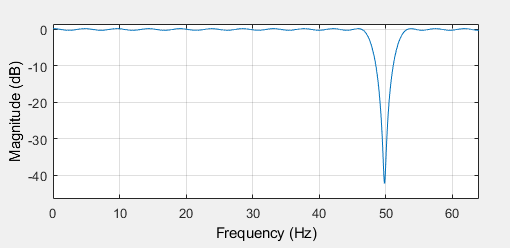
\includegraphics[width=0.5\linewidth]{figures/x1_v11_freqresponse.png}
    \caption{Frequency Response of Filter 1 for Signal $x_3$}
    \label{fig:x1_v11_freqresponse}
\end{figure}

The parameters defining Filter 1 are compiled in Table \ref{tab:x3_v11}.  Typically, the equiripple method will produce the best magnitude response, but in this case, the generalized equiripple method produced a lower order.  The passband ripple was set low so that the information in the data was preserved.

\begin{table}[H]
    \centering
    \begin{tabular}{c|ccccccc}
         Order & Fpass1 & Fstop1 & Fstop2 & Fpass2 & Apass1 & Astop & Apass2 \\ \hline
         56 & $46.6 \unit{Hz}$ & $49.72  \unit{Hz}$ & $49.88  \unit{Hz}$ & $53  \unit{Hz}$ & $0.5  \unit{dB}$ & $40  \unit{dB}$ & $0.5  \unit{dB}$
    \end{tabular}
    \caption{Parameters for Filter 1 for Signal $x_1$}
    \label{tab:x3_v11}
\end{table}

Applying this filter yields the response in Figure \ref{fig:x3_v11}.
\begin{figure}[H]
    \centering
    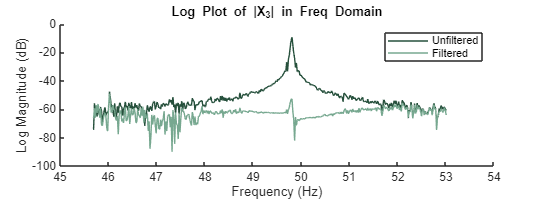
\includegraphics[width=0.5\linewidth]{figures/X3_v11.png}
    \caption{Response of Signal $x_3$ to Filter 1, Order 56}
    \label{fig:x3_v11}
\end{figure}
Notice that the original data is in dark green, while the filtered data is in light green.  It can be seen that this filter removes the interfering spike near $50 \unit{Hz}$ while preserving the rest of the data, with minor adjustments.  In this case, the higher order of 56 is justified, as it better preserves the information found within the signal.  Across the spectrum, Filter 1 removes the interference without adjusting the signal content, as can be seen in Figure \ref{fig:X3_v11_out}.

\begin{figure}[H]
    \centering
    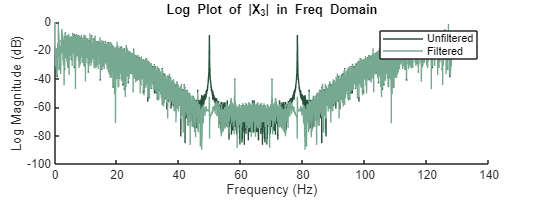
\includegraphics[width=0.5\linewidth]{figures/X3_v11_zoomedout.png}
    \caption{Entire Response of Signal $x_3$ to Filter 1, Order 56}
    \label{fig:X3_v11_out}
\end{figure}


Focusing in on a few heart cycles in Figure \ref{fig:x3_v11_zoom}, we can see that the filter removed most of the contamination resulting from the power line, while preserving what appears to be the information in the data.  This would need to be confirmed by a medical professional.
\begin{figure}[H]
    \centering
    \includegraphics[width=0.5\linewidth]{figures/x3_v11.png}
    \caption{Signal $x_3$ after Filter 1, Order 56, in Time}
    \label{fig:x3_v11_zoom}
\end{figure}

With the interference removed, we are able to analyze the heart rhythm recorded in the ECG.  First, we see that there are 35 R waves present in the first 30 seconds, as seen in Figure \ref{fig:x3_first30}, which allows us to estimate a heart rate of 70 BPM.


\begin{figure}[H]
    \centering
    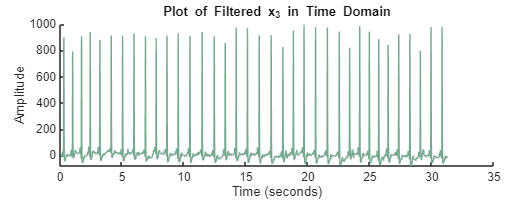
\includegraphics[width=0.5\linewidth]{figures/x3_first30sec.png}
    \caption{Signal $x_3$ over the First 30 Seconds}
    \label{fig:x3_first30}
\end{figure}

Similarly, we count 35 R waves in the last 30 seconds, as seen in Figure \ref{fig:x3_last30}, again allowing us to estimate a heart rate of 70 BPM.

\begin{figure}[H]
    \centering
    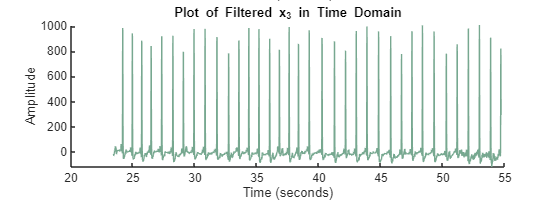
\includegraphics[width=0.5\linewidth]{figures/x3_last30sec.png}
    \caption{Signal $x_3$ over the Last 30 Seconds}
    \label{fig:x3_last30}
\end{figure}

Note that
\begin{align*}
    \frac{70}{1 \unit{min}} \frac{1 \unit{min}}{60 \unit{s}} = 1.167 \unit{Hz}.
\end{align*}
This corresponds to the first, and largest, peak in the data, which can be seen in Figure \ref{fig:x3_avg}
\begin{figure}
    \centering
    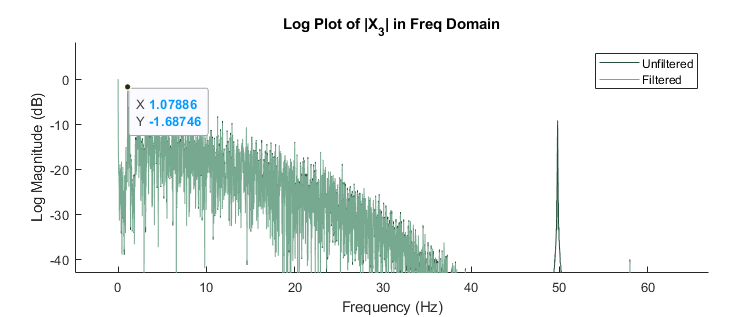
\includegraphics[width=0.5\linewidth]{figures/x3_avg.png}
    \caption{Frequency Spectrum of Signal $x_3$ with Average Heart Rate Highlighted}
    \label{fig:x3_avg}
\end{figure}

Taking a closer look at Figure \ref{fig:x3_v11_zoom}, we can see that there does appear to be a P wave, a very small Q wave, a large and irregular R wave, an S wave, and a T wave.  However, the rhythm between R waves seems irregular, and the  P and T waves are barely present.  Additionally, the amplitude of the R waves is irregular.  This, in many ways, appears similar to the rhythm of atrial fibrillation.  However, this would need to be confirmed by a medical professional, as the interference from the power line could be corrupting the information in the data.